\chapter{Diagrams for Lattice based algorithms}
\label{ch:block_diagrams}

\begin{figure}[ht!]
  \centering
  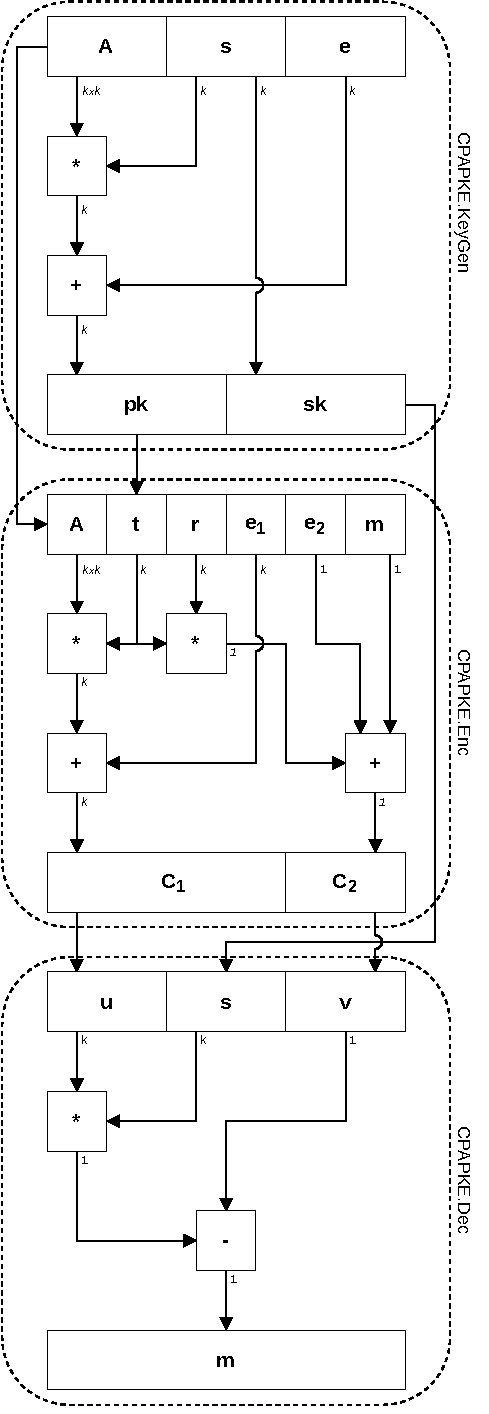
\includegraphics[width=0.484\textwidth]{pictures/kyber_all.pdf}
  \caption{Kyber block scheme}
  \label{img:kyber_all}
\end{figure}

\begin{figure}[ht!]
  \centering
  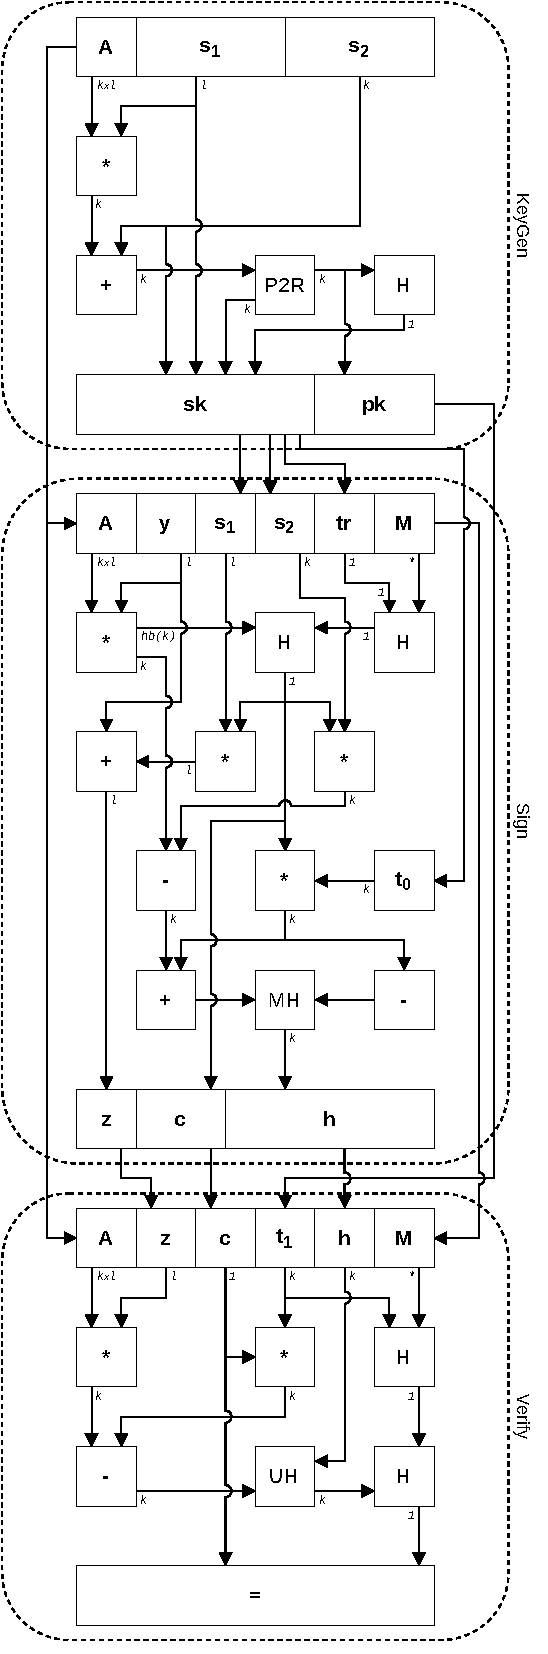
\includegraphics[width=0.497\textwidth]{pictures/dil_all.pdf}
  \caption{Dilithium block scheme}
  \label{img:dil_all}
\end{figure}

\chapter{Go program instructions}
This appendix contains the necessary information for building the go program, running it and then instructions on how to run the provided tests.
\label{ch:go_instructions}
\section{How to build}
Go supports most of the well know operating systems such as Linux, Windows and Mac. However this application only supports the Linux operating system.First of all download the latest version of the go binary from this link
\begin{itemize}
  \item \url{https://go.dev/doc/install}.
\end{itemize}
Once go is installed the binary for this thesis can be built by running
\begin{itemize}
  \item \texttt{go build -v -o pqcom}
\end{itemize}
inside the command line interface. The command also has to be ran inside the root directory of the project. The output of this command should yield a~file named \texttt{pqcom}.
\section{How to run}
Once the binary is built it can be ran just like any other binary. Run with
\begin{itemize}
  \item \texttt{./pqcom}
\end{itemize}
in the command line interface. Refer to chapter \ref{ch:app_capab} for application capabilities or run
\begin{itemize}
  \item \texttt{./pqcom -\--help}
\end{itemize}
to see what commands are available.
\section{Examples}
The benchmarks for implementations of Kyber and Dilithium and for other added post quantum algorithms can be ran without the required configuration files. Here is an example that will run benchmarks for all available algorithms
\begin{itemize}
  \item \texttt{./pqcom benchmark -i 500}
\end{itemize}

Before commands that create quantum resistant connections can be used a configuration file is needed. To easily generate configuration files for booth of the peers run
\begin{itemize}
  \item \texttt{./pqcom config gen}
\end{itemize}
To use different algorithms for the configuration check the section \ref{sec:cmd_config}. Too use a created configuration file use one of the three options defined in section \ref{sec:cmd_app}. Now that configuration files are generated, the application can be used to create connections, for example using the \texttt{chat} command. Firstly the server has to start listening. By default command
\begin{itemize}
  \item \texttt{./pqcom app chat -l --config pqcom\_server\_example.json}
\end{itemize}
will start listening on port \texttt{4040} and on address \texttt{127.0.0.1}. Now a client has to connect by running
\begin{itemize}
  \item \texttt{./pqcom app chat -c --config pqcom\_server\_example.json}
\end{itemize}
where the default remote port is again \texttt{4040} with the IP address \texttt{127.0.0.1}. If everything was done correctly a TUI should open where users can send messages to each other.

\section{How to test}
Tests that check whether the implementations are working correctly can be ran by entering
\begin{itemize}
  \item \texttt{go test -v ./...}
\end{itemize}
into the command line interface in the root directory of the project. There are only two tests than check whether the implementations of the Kyber and Dilithium are functional.

\chapter{Application TUI}
\label{ch:TUI_example}
\object{obr}{pictures/dark.png}{Dark theme application TUI}{img:dark_tui}
\object{obr}{pictures/light.png}{Light theme application TUI}{img:light_tui}
